\chapter{Tape Sessions and Sub-processes}

\section{Introduction}

The program {\tt cta-taped} is a daemon managing the tape drive and transferring data from tape to drive. The daemon has
two levels of processes:
\begin{description}
\item[The Daemon Process:] a single threaded sub-process manager which does not have any external connectivity. The
Daemon Process is very simple and has a long lifetime (in the order of months).
\item[Sub-processes:] implement external connectivity. Sub-processes can be multi-threaded. They have a short lifetime
with regular restarts, to limit the consequences of memory leaks or other potential bugs in third-party tape libraries.
\end{description}

There are several types of Sub-process. The main Sub-process is the drive sub-process (see below).

\begin{alertbox}
Other possible sub-processes:
\begin{itemize}
\item Labelling process?
\item Drive cleaning process?
\item Verification process? Perhaps not necessary as a read-only Drive process could do the job?
\end{itemize}
Are these part of the Drive sub-process or are they separate processes launched by the Drive sub-process?
\end{alertbox}

\clearpage

\section{Drive sub-process}

One Drive sub-process is launched per drive in the tape server. The Drive sub-process executes one mount and then exits.

The daemon then restarts a new Drive sub-process instance, passing in the previous instances' exit status. Based on this
status from the previous run, the session could become either:
\begin{description}
\item[A Cleanup Session:] any potentially still-mounted tape is removed from the drive, or
\item[A Scheduling Session:] Scheduling can lead to Archive, Retrieve or Labelling sessions.
\end{description}

The tape session types and state changes are shown in Figure~\ref{statediag}.

\begin{figure}[h!]
\centering
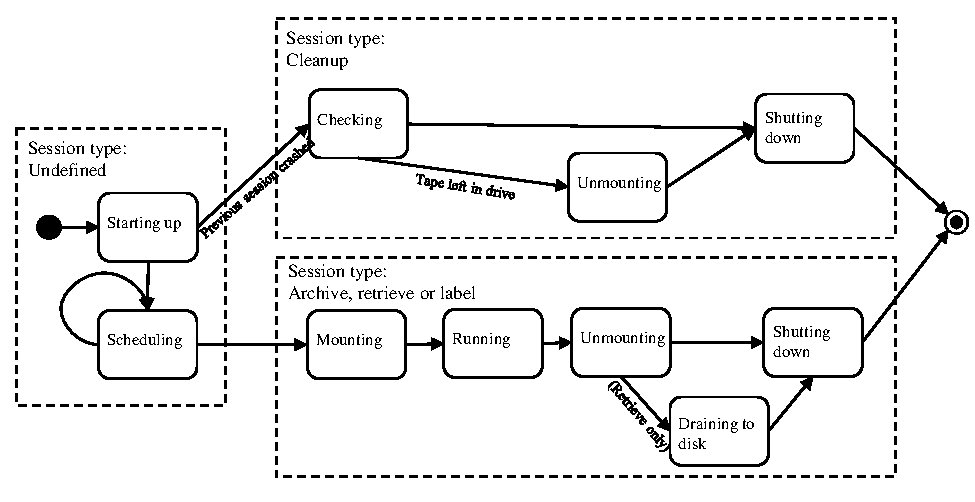
\includegraphics{CTA_tape_session_states}
\caption{Tape sessions state diagram}
\label{statediag}
\end{figure}

